\documentclass[11pt, titlepage]{article}

\usepackage[margin=1in]{geometry}
\usepackage[strict]{changepage}
\usepackage{float}
\usepackage{fancyhdr}
\usepackage{mhchem}
\usepackage{siunitx}
\usepackage{wrapfig, booktabs}
\usepackage{enumitem}
\usepackage{caption}
\usepackage{commath}
\usepackage{amsmath}
\usepackage[hang]{footmisc}
\usepackage{multicol}
\usepackage{amsfonts}
\usepackage{mathrsfs}
\usepackage{mathtools}
\usepackage{tikz}

% my imports
\usepackage[most]{tcolorbox}
\usepackage{hyperref}
\hypersetup{
    colorlinks,
    citecolor=black,
    filecolor=black,
    linkcolor=black,
    urlcolor=black
}

\newcommand{\experimentDate}{\today}
\newcommand{\className}{CSE 371}
\newcommand{\assignmentname}{Lab 6 Proposal}
\author{Donovan Clay (ID: 2276005), Cameron Jennings (ID: 2029631)}
\newcommand{\authorLastName}{Clay, Jennings}
\title{\assignmentname}

\date{\parbox{\linewidth}{\centering
\experimentDate
  \endgraf\bigskip
  \className\
}}

\pagestyle{fancy}
\fancyhf{}
\setlength{\headheight}{13.59999pt}
\rhead{\authorLastName\ \thepage}
% \lhead{\experimentShortName}
\lhead{\hyperref[beginning]{\assignmentname}}
\cfoot{\className\ -- \assignmentname}

\usepackage{color}
\usepackage{sectsty}

\definecolor{WordSectionBlue}{RGB}{30, 90, 147}

\allsectionsfont{\color{WordSectionBlue}}

\tcbuselibrary{breakable}

\begin{document}
	\maketitle
 
    \setcounter{tocdepth}{2}
    \begin{center}
        \tableofcontents\label{beginning}
    \end{center}
    \newpage
    
    \section{Major Project Behavior}
        \begin{tcolorbox}
            Our project will be recreating a simple version of Space Invaders / Galaca. This will take user input from an N8 controller and output display via the VGA. Space invaders is a single player game against the ``bot'' enemies. The player controls a spaceship with the N8 controller. They can move the ship left and right and can shoot lasers forward. The aliens move left and right and as the game continues, they advance towards the player's ship. The aliens can also shoot lasers. If the player gets hit by an alien laser, they die and lose the game. If an alien gets hit by the player's laser, they die and disappear. The player also loses of the aliens touch the player. The player wins when they kill all the aliens.
        \end{tcolorbox}
    \section{Top Level Block Diagram}
        \begin{tcolorbox}
            \begin{center}
                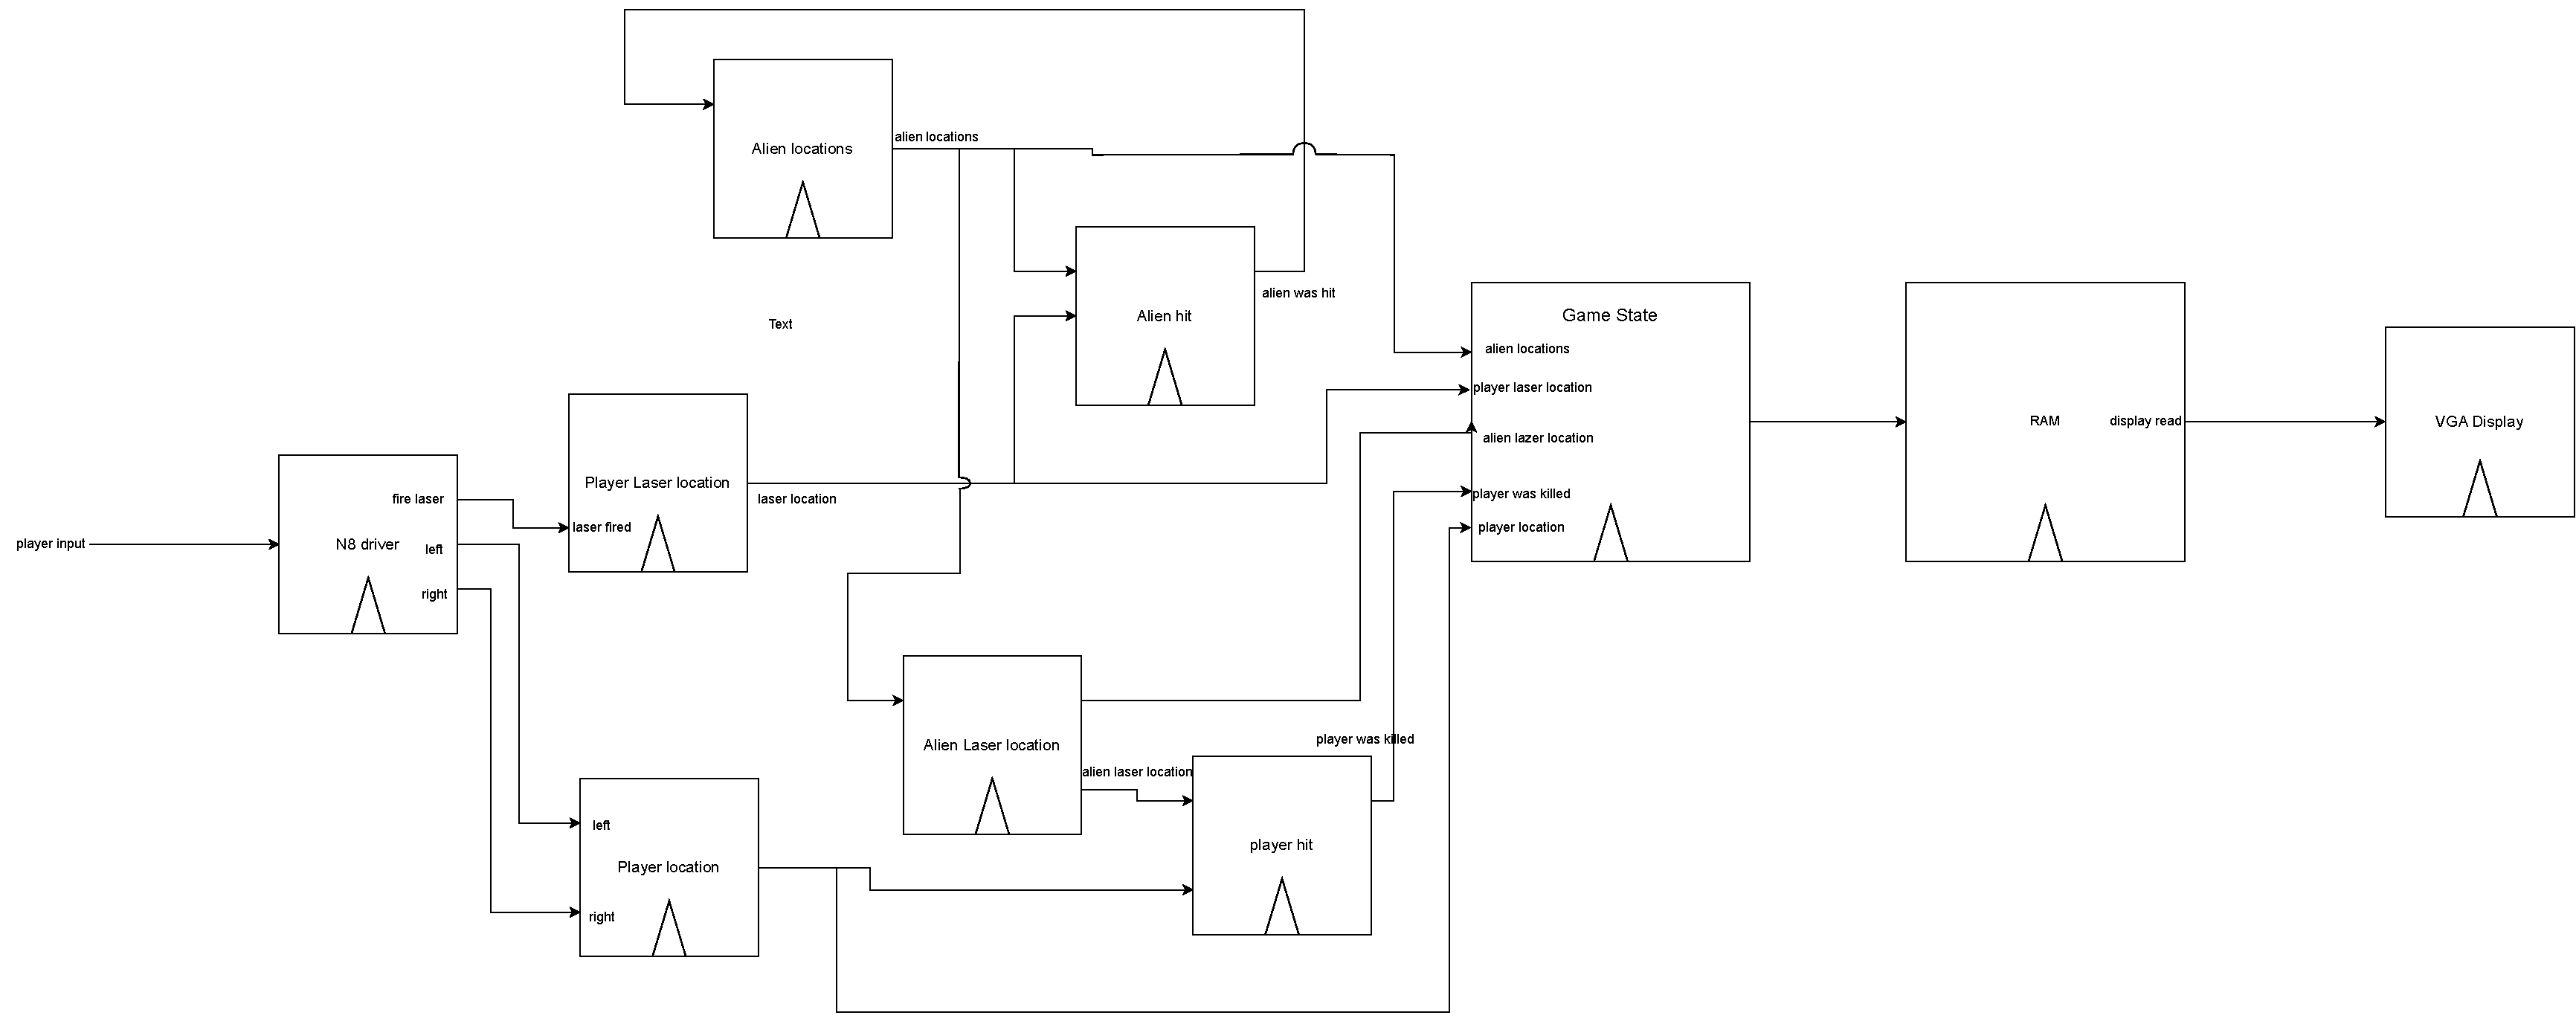
\includegraphics[scale=0.24]{Lab 6 Proposal.pdf}
            \end{center}
        \end{tcolorbox}
\end{document}
